% Admissible set on two planes through theta: a rectangle for h = e_3, a polygon for h = (1,1,0,0,0).
% Source of the figure, typeset in the paper's own fonts (T1, Latin Modern, 11pt) at the paper's text
% width (6.5in), so \includegraphics does not rescale it. Illustrates CLH-2; it adds no assertion.
% Every coordinate and printed number is read from values that Lean evaluated (Conj43.crossEdges, the gaps, the plane and its half-plane clipping);
% inputs: f-bar=(3,5,1,2,4), theta/pi=(0,0.1,0.7,0.3,0.8).
% SHA-256 (first 16 hex digits) of the output lines the values come from: adm_e3 a6b38b7b803df931, adm_diag ae66ce085bebec1f.
% Real-valued quantities are floating-point values computed in Lean from the paper's formulas.
% Build: pdflatex <this file> && pdftocairo -svg <this file>.pdf <this file>.svg
\documentclass[11pt]{standalone}
\usepackage[T1]{fontenc}
\usepackage{lmodern}
\usepackage{amsmath,amssymb}
\usepackage{tikz}
\usetikzlibrary{arrows.meta,positioning,calc}

% the palette of the paper's other figures: blue solid for the first curve or strand, ochre dashed for the second
\definecolor{ink}{HTML}{233740}
\definecolor{muted}{HTML}{65757D}
\definecolor{pblue}{HTML}{0072B2}
\definecolor{qochre}{HTML}{B87827}

\tikzset{
  frm/.style={draw=muted, line width=0.5pt},
  axl/.style={draw=muted!70, line width=0.4pt},
  crvP/.style={draw=pblue, line width=1.1pt, line join=round},
  crvQ/.style={draw=qochre, line width=1.1pt, dash pattern=on 4pt off 1.6pt},
  drop/.style={draw=muted, line width=0.4pt, dash pattern=on 1pt off 1.4pt},
  dotQ/.style={circle, fill=qochre, draw=qochre, inner sep=0pt, minimum size=4.2pt},
  dotP/.style={circle, fill=pblue, draw=pblue, inner sep=0pt, minimum size=4.2pt},
  openQ/.style={circle, fill=white, draw=qochre, line width=0.8pt, inner sep=0pt, minimum size=4.2pt},
  lab/.style={font=\footnotesize, inner sep=1.5pt, text=ink},
  labm/.style={font=\small, inner sep=1.5pt, text=ink},
  labQ/.style={font=\footnotesize, inner sep=1.5pt, text=qochre},
  labP/.style={font=\footnotesize, inner sep=1.5pt, text=pblue},
  tick/.style={font=\footnotesize, inner sep=1.2pt, text=muted},
  vtx/.style={circle, draw=ink, fill=white, line width=0.6pt, inner sep=0pt, minimum size=15pt, font=\small, text=ink},
  arrP/.style={pblue, line width=1.0pt, -{Stealth[length=5pt,width=4.2pt]}},
}

\begin{document}
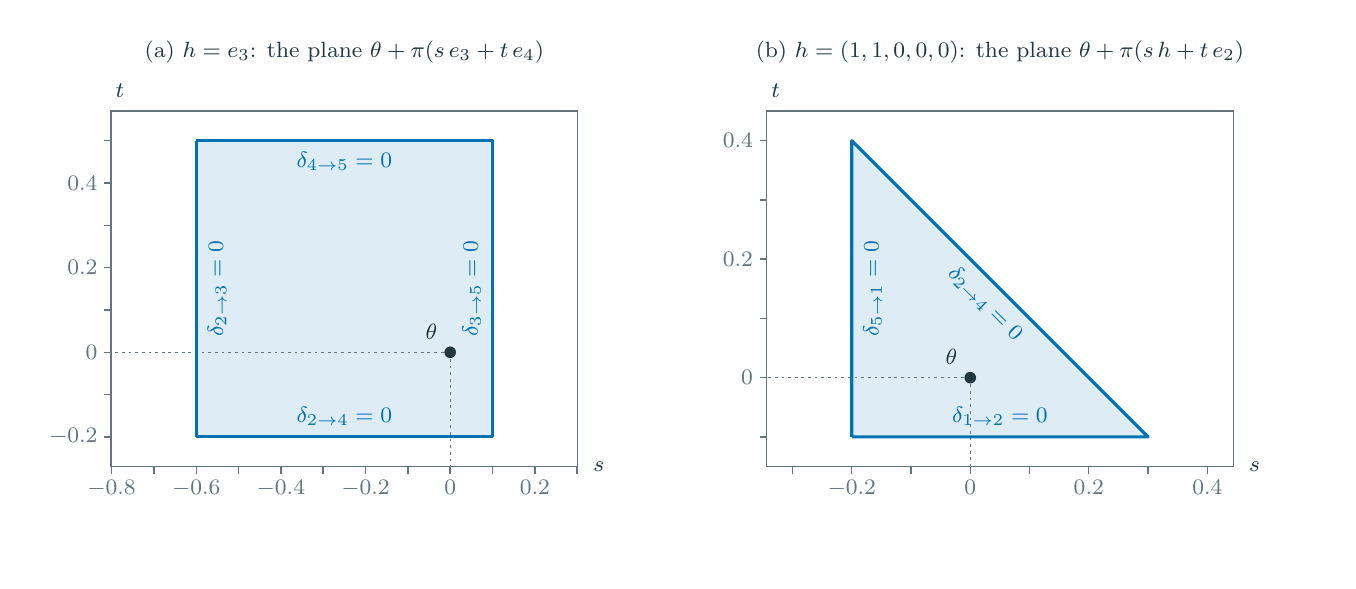
\begin{tikzpicture}[x=1bp,y=1bp]
\useasboundingbox (0,0) rectangle (468.005,192.0025);
% map Aa 152.0952 75.1429 152.3810 152.3810
\draw[frm] (30.00,34.00) rectangle (198.00,162.00);
\draw[frm] (30.19,34.00) -- (30.19,31.50);
\node[tick, anchor=north] at (30.19,30.50) {$-0.8$};
\draw[frm] (45.43,34.00) -- (45.43,31.50);
\draw[frm] (60.67,34.00) -- (60.67,31.50);
\node[tick, anchor=north] at (60.67,30.50) {$-0.6$};
\draw[frm] (75.90,34.00) -- (75.90,31.50);
\draw[frm] (91.14,34.00) -- (91.14,31.50);
\node[tick, anchor=north] at (91.14,30.50) {$-0.4$};
\draw[frm] (106.38,34.00) -- (106.38,31.50);
\draw[frm] (121.62,34.00) -- (121.62,31.50);
\node[tick, anchor=north] at (121.62,30.50) {$-0.2$};
\draw[frm] (136.86,34.00) -- (136.86,31.50);
\draw[frm] (152.10,34.00) -- (152.10,31.50);
\node[tick, anchor=north] at (152.10,30.50) {$0$};
\draw[frm] (167.33,34.00) -- (167.33,31.50);
\draw[frm] (182.57,34.00) -- (182.57,31.50);
\node[tick, anchor=north] at (182.57,30.50) {$0.2$};
\draw[frm] (197.81,34.00) -- (197.81,31.50);
\draw[frm] (30.00,44.67) -- (27.50,44.67);
\node[tick, anchor=east] at (26.50,44.67) {$-0.2$};
\draw[frm] (30.00,59.90) -- (27.50,59.90);
\draw[frm] (30.00,75.14) -- (27.50,75.14);
\node[tick, anchor=east] at (26.50,75.14) {$0$};
\draw[frm] (30.00,90.38) -- (27.50,90.38);
\draw[frm] (30.00,105.62) -- (27.50,105.62);
\node[tick, anchor=east] at (26.50,105.62) {$0.2$};
\draw[frm] (30.00,120.86) -- (27.50,120.86);
\draw[frm] (30.00,136.10) -- (27.50,136.10);
\node[tick, anchor=east] at (26.50,136.10) {$0.4$};
\draw[frm] (30.00,151.33) -- (27.50,151.33);
\node[lab, anchor=west] at (202.00,34.00) {$s$};
\node[lab, anchor=south west] at (30.00,165.00) {$t$};
\fill[pblue!13] (60.67,151.33) -- (60.67,44.67) -- (167.33,44.67) -- (167.33,151.33) -- cycle;
\draw[drop] (152.10,75.14) -- (152.10,34.00);
\draw[drop] (152.10,75.14) -- (30.00,75.14);
\draw[crvP] (60.67,151.33) -- (60.67,44.67) -- (167.33,44.67) -- (167.33,151.33) -- (60.67,151.33); %poly Aa region
\node[labP, anchor=center, rotate=90.00] at (68.17,98.00) {$\delta_{2{\to}3}=0$}; %val edge 0 2→3
\node[labP, anchor=center, rotate=0.00] at (114.00,52.17) {$\delta_{2{\to}4}=0$}; %val edge 1 2→4
\node[labP, anchor=center, rotate=90.00] at (159.83,98.00) {$\delta_{3{\to}5}=0$}; %val edge 2 3→5
\node[labP, anchor=center, rotate=0.00] at (114.00,143.83) {$\delta_{4{\to}5}=0$}; %val edge 3 4→5
\node[circle, fill=ink, inner sep=0pt, minimum size=4.2pt] at (152.10,75.14) {}; %mark Aa theta 0
\node[lab, anchor=south east] at (149.10,78.14) {$\theta$};
\node[lab, anchor=north] at (114.00,189.00) {(a) $h=e_3$: the plane $\theta+\pi(s\,e_3+t\,e_4)$};
% map Ab 339.3333 66.0000 213.3333 213.3333
\draw[frm] (266.00,34.00) rectangle (434.00,162.00);
\draw[frm] (275.33,34.00) -- (275.33,31.50);
\draw[frm] (296.67,34.00) -- (296.67,31.50);
\node[tick, anchor=north] at (296.67,30.50) {$-0.2$};
\draw[frm] (318.00,34.00) -- (318.00,31.50);
\draw[frm] (339.33,34.00) -- (339.33,31.50);
\node[tick, anchor=north] at (339.33,30.50) {$0$};
\draw[frm] (360.67,34.00) -- (360.67,31.50);
\draw[frm] (382.00,34.00) -- (382.00,31.50);
\node[tick, anchor=north] at (382.00,30.50) {$0.2$};
\draw[frm] (403.33,34.00) -- (403.33,31.50);
\draw[frm] (424.67,34.00) -- (424.67,31.50);
\node[tick, anchor=north] at (424.67,30.50) {$0.4$};
\draw[frm] (266.00,44.67) -- (263.50,44.67);
\draw[frm] (266.00,66.00) -- (263.50,66.00);
\node[tick, anchor=east] at (262.50,66.00) {$0$};
\draw[frm] (266.00,87.33) -- (263.50,87.33);
\draw[frm] (266.00,108.67) -- (263.50,108.67);
\node[tick, anchor=east] at (262.50,108.67) {$0.2$};
\draw[frm] (266.00,130.00) -- (263.50,130.00);
\draw[frm] (266.00,151.33) -- (263.50,151.33);
\node[tick, anchor=east] at (262.50,151.33) {$0.4$};
\node[lab, anchor=west] at (438.00,34.00) {$s$};
\node[lab, anchor=south west] at (266.00,165.00) {$t$};
\fill[pblue!13] (296.67,44.67) -- (403.33,44.67) -- (296.67,151.33) -- cycle;
\draw[drop] (339.33,66.00) -- (339.33,34.00);
\draw[drop] (339.33,66.00) -- (266.00,66.00);
\draw[crvP] (296.67,44.67) -- (403.33,44.67) -- (296.67,151.33) -- (296.67,44.67); %poly Ab region
\node[labP, anchor=center, rotate=0.00] at (350.00,52.17) {$\delta_{1{\to}2}=0$}; %val edge 0 1→2
\node[labP, anchor=center, rotate=-45.00] at (344.70,92.70) {$\delta_{2{\to}4}=0$}; %val edge 1 2→4
\node[labP, anchor=center, rotate=90.00] at (304.17,98.00) {$\delta_{5{\to}1}=0$}; %val edge 2 5→1
\node[circle, fill=ink, inner sep=0pt, minimum size=4.2pt] at (339.33,66.00) {}; %mark Ab theta 0
\node[lab, anchor=south east] at (336.33,69.00) {$\theta$};
\node[lab, anchor=north] at (350.00,189.00) {(b) $h=(1,1,0,0,0)$: the plane $\theta+\pi(s\,h+t\,e_2)$};
\end{tikzpicture}
\end{document}
